\section{Study Application}
This section will describe the study application in terms of components and will illustrate how the application looked.

\subsection{Installing the Application}
The application was only released on iOS as previously mentioned and was distributed exclusively via Apple's TestFlight service. 

Once the user had such an invitation the installation process was the following: 
\begin{itemize}
    
    \item The user installs the TestFlight application via the App Store.
    
    \item The user installs the Mobility Study app via the TestFlight application.
    
    \item Once the Mobility Study app is installed, it will ask for permission to track the user's location as well as sending the user notifications. 
    
\end{itemize}
The location tracking is necessary for the collection of location data whereas notifications are not necessary, but do help the user be reminded to fill out a daily questionnaire. An installation manual (see Appendix \ref{appendix:installation}) was provided to the participants to ensure the applications were set up correctly and the installation process is shown in Figure \ref{fig:screens-install}.

\begin{figure}
    \centering
    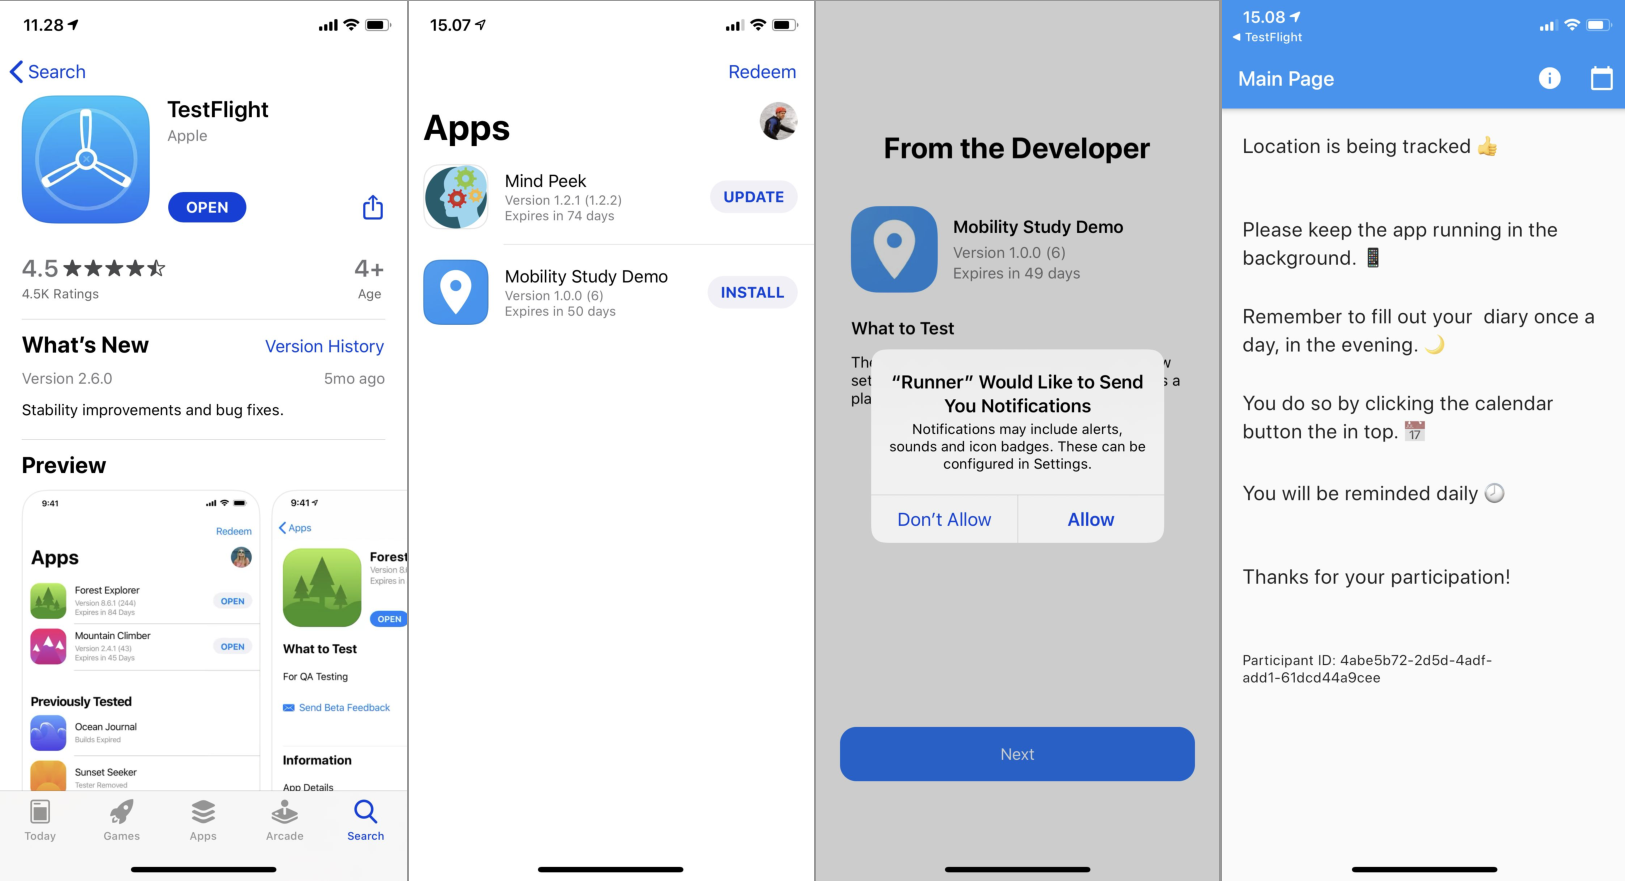
\includegraphics[width=\textwidth]{images/app_imgs/screens-install.pdf}
    \caption{The initial installation- and setup process for the user}
    \label{fig:screens-install}
\end{figure}

\subsection{App Screens}
The Main Page of the application displays a list of instructions and does not have any interesting functionality. From the main screen, it is possible to navigate to the Info Page and the Diary Page, from the navigation bar at the top. The Info Page is made to inform the user of how the data will be used, and an email to contact the researcher in case of any questions. \\

The Diary Page contains the questionnaire the user has to answer daily. The user can either navigate to this page themselves or tap the notification they receive each evening. The four questions can be answered by pressing the \textit{Pick an Answer}-button which will show a wheel of possible values to pick an answer from. Once all questions have been answered, the submit button will be enabled. Submitting the answers will upload the answers to a server, and store them on the device as well. When storing is done, the last screen will appear which informs the user the answers have been saved and thanks them for their contribution.

\begin{figure}
    \centering
    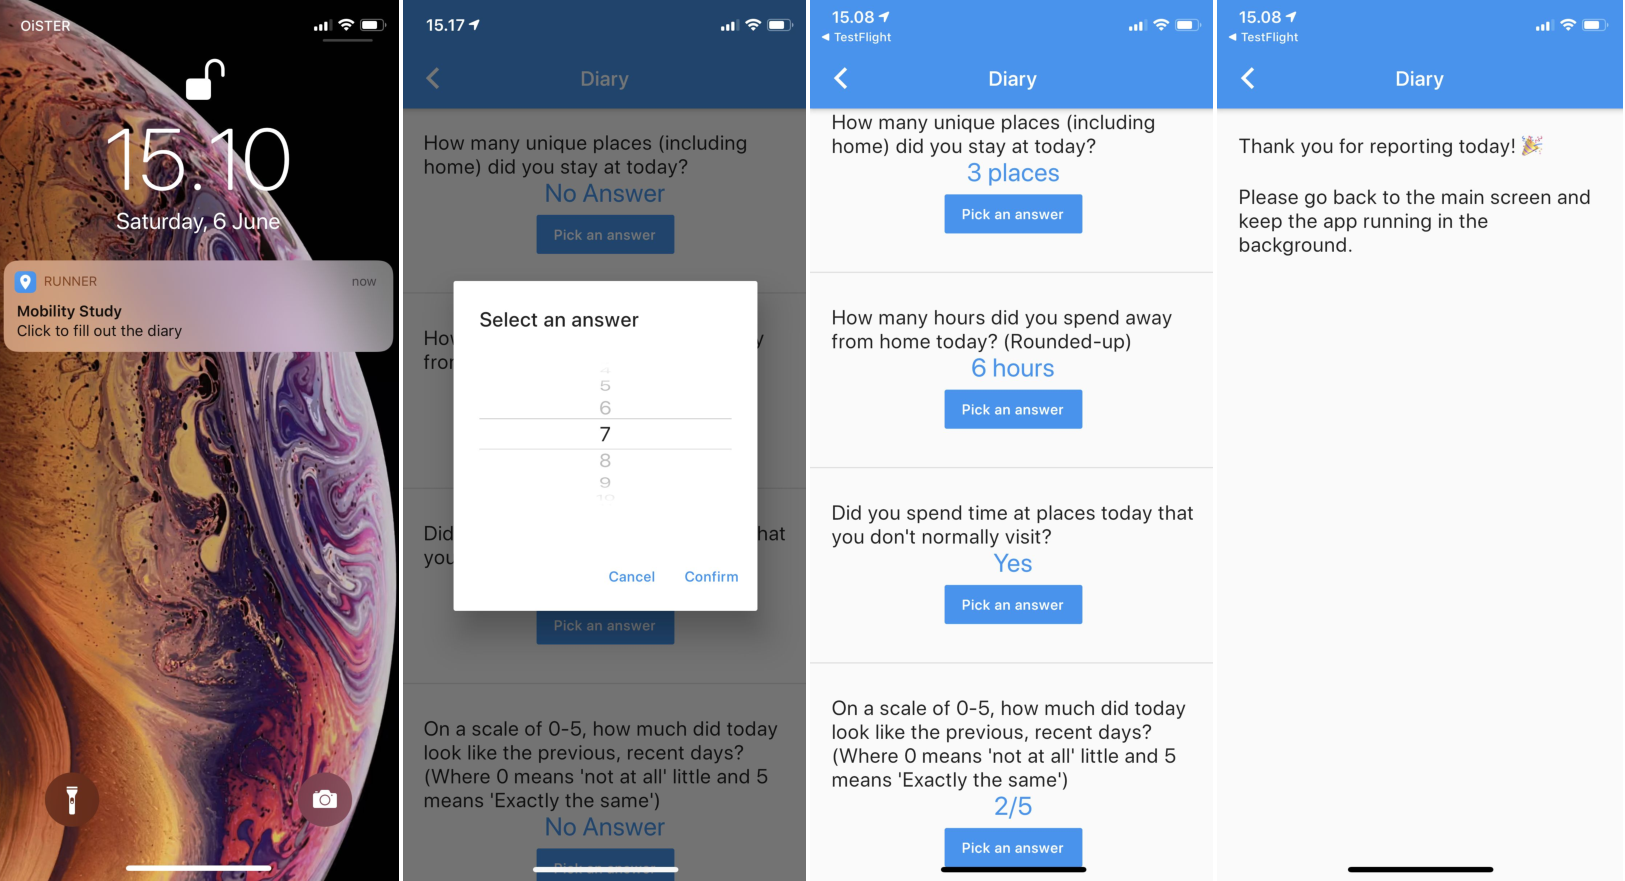
\includegraphics[width=\textwidth]{images/app_imgs/screens-answers.pdf}
    \caption{The different screens which the user is taken through for submitting answers}
    \label{fig:screens-answers}
\end{figure}

\subsection{Displaying Features}
An initial version of the application included a display of the real-time calculated features, which were recalculated each time a button was pressed. It was decided to not display the features in the final version for the study since they would influence the answers given by the users. This display of features may be relevant for a real-world application where it makes sense to inform the user of the feature values, such as how much they have stayed at home.

\begin{figure}
    \centering
    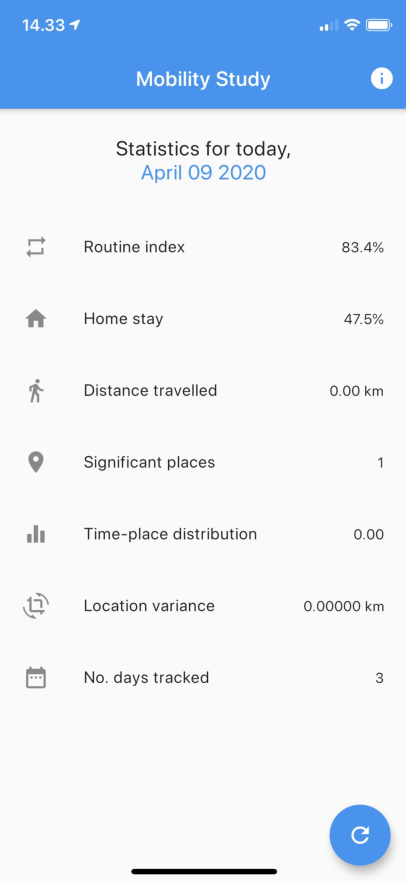
\includegraphics[width=0.3\textwidth]{images/app_imgs/screens-features.pdf}
    \caption{An early iteration of the study app in which the feature values were shown}
    \label{fig:app-features-screen}
\end{figure}

\subsection{Data Storage}
To store the data from the study online, such that it could later be extracted for data analysis, a Firebase file storage server was used for uploading files multiple times daily. Concretely, the LocationSamples, Stops, and Moves were stored locally on the device. Whenever a Feature calculation was triggered, the calculated MobilityContext was serialized and uploaded as a file, in addition to the data points for the day and all Stops and Moves on the phone for the last 28 days (see Chapter \ref{chapter:03}).